\documentclass[11pt,a4paper]{article}
\usepackage{fontspec}
\setmainfont{TeX Gyre Termes}
\setmonofont{Latin Modern Mono}[Scale=0.95]
\usepackage[margin=2.6cm,top=2.8cm,bottom=2.8cm]{geometry}
\usepackage{graphicx,booktabs,amsmath,xcolor,listings,fancyhdr,caption,titlesec,microtype,enumitem}
\usepackage[hidelinks]{hyperref}
\usepackage{float}
\usepackage[round,authoryear]{natbib}

\definecolor{codebg}{HTML}{F5F5F2}
\definecolor{codekw}{HTML}{1C5CAB}
\definecolor{codecm}{HTML}{6E6D68}
\lstset{language=Python,basicstyle=\ttfamily\small,backgroundcolor=\color{codebg},
  keywordstyle=\color{codekw},commentstyle=\color{codecm}\itshape,
  frame=none,xleftmargin=1em,framexleftmargin=1em,aboveskip=8pt,belowskip=8pt,
  columns=fullflexible,keepspaces=true,showstringspaces=false}

\captionsetup{font={small,it},labelfont={small,it},justification=centering}
\titleformat{\section}{\large\bfseries}{\thesection.}{0.5em}{}
\titleformat{\subsection}{\normalsize\bfseries}{\thesubsection}{0.5em}{}
\titlespacing*{\section}{0pt}{14pt}{6pt}
\titlespacing*{\subsection}{0pt}{10pt}{4pt}
\setlength{\parskip}{5pt}\setlength{\parindent}{0pt}

\pagestyle{fancy}\fancyhf{}
\fancyhead[L]{\small\itshape The Fiscal Footprint of Italy's Superbonus 110\%}
\fancyhead[R]{\small\itshape Ettore Mancuso}
\fancyfoot[C]{\small\thepage}
\renewcommand{\headrulewidth}{0.4pt}\renewcommand{\footrulewidth}{0.4pt}

\newcommand{\pct}{\%}

\begin{document}
\thispagestyle{empty}
\begin{center}
{\LARGE\bfseries Paying for the Renovation Boom:\\[4pt] The Fiscal Footprint of Italy's Superbonus 110\%}\\[10pt]
{\large\itshape A data-driven assessment of take-up, deficit accounting, debt timing and\\ the multiplier the scheme would have needed}\\[22pt]
{\large Ettore Mancuso}\\[1pt]
\href{mailto:ettoremancuso6@gmail.com}{ettoremancuso6@gmail.com}\\[1pt]
September 2026
\end{center}
\vspace{16pt}

\section*{Abstract}
Between 2020 and 2025 Italy financed the renovation of about half a million buildings through the Superbonus 110\%, a tax credit worth more than the cost of the works and, until 2023, freely transferable to third parties. I build a small dataset from ENEA, Istat, the European Commission and recent empirical studies, with a source for every number, and run four exercises on it in Python. The first documents take-up: certified investment grew by about EUR~3.8 billion per month between mid-2022 and end-2023 and stalled once transferability was removed, reaching EUR~124 billion. The second decomposes the deficit: building credits account for roughly 4 of the 7.2 points of GDP of net borrowing in 2023, and removing them would have left the deficit near the 3\% reference value. In the third, a stylised cash-offset model shows why the same cost reaches public debt years after it reaches the deficit: about 2\% of GDP per year is absorbed in 2024--2026, and the profile barely moves under different instalment assumptions. The fourth is a break-even analysis. It shows that, given the deadweight shares estimated by the Bank of Italy and the Treasury (27--38\%), each additional euro of construction would have had to raise GDP by 1.36--1.60 euro for the scheme to break even in output terms, and by more than 3 euro to pay for itself through tax revenue. The stimulus worked, but it was expensive, and its design gave nobody a reason to control cost.

\medskip
\textbf{Keywords:} fiscal policy, tax credits, Superbonus, fiscal multiplier, deadweight loss, public debt, government accounting, Italy

\textbf{JEL classification:} E62, H24, H62, H63, R31, Q48

\section{Introduction}
In May 2020, with Italian GDP heading for a contraction of 8.9\% for the year, the government introduced a home-renovation incentive meant to revive a construction sector that had stagnated for more than a decade while advancing the energy transition \citep{capone2026}. The Superbonus 110\% had two unusual features: the subsidy exceeded the full cost of the works, and the resulting credit could be sold to a bank or converted into an up-front discount on the invoice. Planned as a one-year measure, it was extended repeatedly and survived three governments. Together with the parallel façade bonus, its total fiscal cost is estimated at about EUR~220 billion, some EUR~150 billion above initial projections \citep{capone2026}.

The scheme has already generated a substantial literature. Counterfactual studies by the Bank of Italy and the Treasury estimate how much investment was additional \citep{accetturo2026,mef_wp}; Corsello and Ercolani quantify its effect on construction costs \citep{corsello2024,corsello2025}; and institutional reviews assess its implications for public finances \citep{codogno2024,imf2024}. I do not attempt a new causal estimate. My aim is narrower. I put the publicly available numbers into one reproducible dataset and apply tools from an undergraduate economics programme, namely national-accounts identities, a small simulation and a break-even condition for the fiscal multiplier. The paper asks three questions:

\begin{enumerate}[leftmargin=1.5em,itemsep=2pt]
\item How large was the scheme's footprint on the deficit, and how much did the accounting treatment matter?
\item Why does the cost of the scheme reach public debt years after it appears in the deficit?
\item Given the estimated deadweight, how large a multiplier would the scheme have needed to break even, or to ``pay for itself''?
\end{enumerate}

Section~2 summarises the policy design. Section~3 describes the data and methods. Section~4 presents the results, Section~5 relates them to the literature, Section~6 discusses limitations and Section~7 concludes. All figures and tables are produced by an accompanying Jupyter notebook.

\section{How the scheme worked}
Italy had offered tax deductions for home renovations since the late 1990s, with rates rising to 65--75\% for energy-efficiency work after 2007 \citep{capone2026}. The Superbonus broke with this tradition in two ways. First, the subsidy rate of 110\% covered the entire cost of eligible works plus an implicit financing margin, recovered in four or five annual instalments. Second, the credit was transferable: a household without enough tax liability could sell it, and a construction firm could offer a discount on the invoice and take over the credit itself.

Transferability was meant to include liquidity-constrained households. Its side effect was to remove the usual conflict of interest between buyer and seller, since a homeowner reimbursed for more than the full bill has no reason to negotiate the price. It also changed the statistical nature of the credit. Under the rules of the Eurostat \textit{Manual on Government Deficit and Debt}, a credit that can be transferred or used regardless of the holder's tax liability is a \textit{payable} tax credit: it must be recorded in full as government expenditure in the year the work is carried out, rather than as lower revenue in the years in which it is used \citep{capone2026,istat2023eurostat}. From 2022 onwards the rules were tightened repeatedly; transferability for new projects was abolished in 2023--24 and the rate was cut to 70\% for 2024 and 65\% for 2025 \citep{capone2026}.

\section{Data and methods}
\subsection{Data}
Because no single database covers the scheme, the analysis relies on four hand-collected files, each row carrying its source (Table~\ref{tab:data}). All values are in nominal euros or percent of GDP. Two data issues deserve mention. The ENEA series changes definition over time (projects admitted, total investment, investment admitted to deduction); the September 2021 observation measures concluded works only and is therefore shown separately. The deficit series combines the latest available Istat vintage for each year with the first published estimates for 2020--2022, which allows the effect of the reclassification to be displayed.

\begin{table}[H]\centering\small
\caption{Data used in the analysis.}\label{tab:data}
\begin{tabular}{p{3.6cm}p{5.0cm}p{5.1cm}}
\toprule
File & Content & Sources \\
\midrule
\texttt{enea\_takeup.csv} & Cumulative certified investment and number of buildings, 2021--2025 & ENEA monthly reports, via \citet{upb2024}, BUILD UP, Eurofound, Edilportale, BibLus, Teleborsa \\
\texttt{enea\_composition} & Certifications and investment by building type, 30 Sep 2025 & ENEA via \citet{edilportale2025} \\
\texttt{deficit.csv} & Net borrowing 2019--2025, first estimates, accrued cost of building credits & Istat releases 2023--2026; \citet{agi2023}; \citet{corsello2025}; \citet{ec2025} \\
\texttt{literature\_estimates} & Take-up and deadweight estimates & \citet{accetturo2026}; \citet{mef_wp} \\
\bottomrule
\end{tabular}
\end{table}

\subsection{Deficit decomposition}
Net borrowing is split into the accrued cost of building credits and the remainder. The credit component follows \citet{corsello2025}, who put it at almost 1\%, 3\% and 4\% of GDP in 2021, 2022 and 2023; the 2024 value (0.5\%) is derived from the European Commission's statement that lower renovation credits reduced the deficit by about 3.5 points between 2023 and 2024 \citep{ec2025}. The remainder is an accounting residual, not a counterfactual: without the scheme, GDP and tax revenue would also have been different.

\subsection{Cash-offset simulation}
Let $A_t$ be the credits accrued in year $t$ (in percent of GDP) and $n_t$ the number of equal annual instalments in which that vintage is used, starting in $t+1$. The cash cost in year $s$, which is what raises the borrowing requirement and therefore debt, is
\begin{equation}
C_s=\sum_{t}\frac{A_t}{n_t}\,\mathbf{1}\{\,t< s\le t+n_t\,\}.
\end{equation}
The baseline uses five instalments for 2021 works, four for 2022--23 and ten for 2024, the rule introduced that year \citep{imf2024}. GDP is held constant, so the model describes timing rather than providing a forecast. The complete function is reproduced below.

\begin{lstlisting}
def cash_profile(accruals, instalments, start_lag=1, horizon=(2021, 2034)):
    # Spread each vintage of payable tax credits into equal annual offsets.
    # accruals: {year: % of GDP accrued}; instalments: {year: n instalments}
    years = np.arange(horizon[0], horizon[1] + 1)
    cash = pd.Series(0.0, index=years)
    for t, a in accruals.items():
        n = instalments[t]
        for k in range(n):
            s = t + start_lag + k
            if s in cash.index:
                cash[s] += a / n
    return cash
\end{lstlisting}

\subsection{Break-even multiplier}
Let $s$ be the fiscal cost per euro of subsidised work, $d$ the deadweight share (subsidised spending that would have occurred anyway) and $k$ the GDP effect of one euro of additional construction spending, including indirect and induced effects. The implied multiplier on public money is
\begin{equation}
m=\frac{k\,(1-d)}{s}.
\end{equation}
The scheme breaks even in output terms when $m\ge 1$, and it ``pays for itself'' when the extra tax revenue covers the cost, $\tau m\ge1$, where $\tau$ is the ratio of taxes to GDP. I set $s=1$, a blend of the 110\% Superbonus and the 90\%/60\% façade bonus, and $\tau=42.7\%$, Istat's 2022 tax burden \citep{istat2023conti}. Solving for $k$ gives the break-even thresholds $k^{*}=s/(1-d)$ and $k^{**}=s/[\tau(1-d)]$.

\section{Results}
\subsection{Take-up dynamics}
Figure~\ref{fig:takeup} shows the cumulative investment certified to ENEA. Between July 2022 and December 2023 the stock rose from EUR~40 to EUR~104 billion, about EUR~3.8 billion per month. After transferability was abolished for new projects and the rate was cut, growth fell to about EUR~0.6 billion per month in 2025, and the series converged to roughly EUR~124 billion across 502,544 buildings at the end of 2025. The pattern suggests that transferability, rather than the headline rate alone, was what made the scheme scale.

\begin{figure}[htbp]\centering
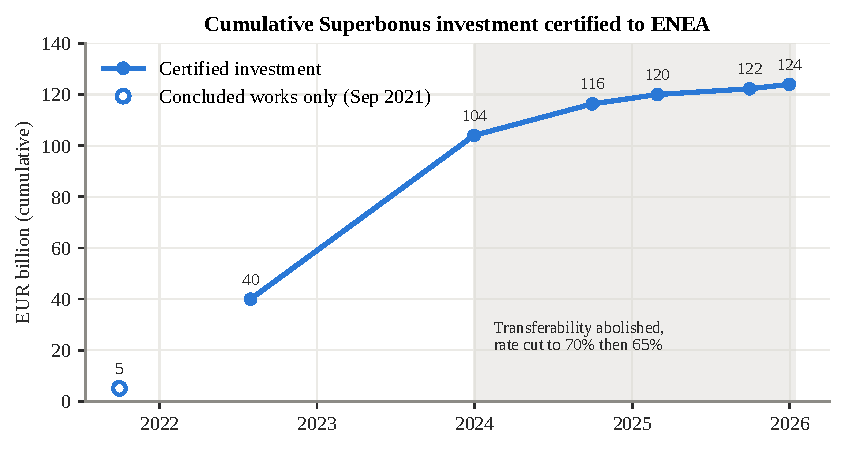
\includegraphics[width=0.86\textwidth]{../figures/fig1_takeup.pdf}
\caption{Cumulative Superbonus investment certified to ENEA. The hollow marker measures concluded works only and is not directly comparable with later points.}\label{fig:takeup}
\end{figure}

Figure~\ref{fig:comp} compares each building type's share of certifications with its share of investment. Condominiums account for 28\% of certifications but 68\% of investment, with an average of about EUR~600,000 per certification against roughly EUR~110,000 for single-family homes. Money was therefore concentrated in a minority of large projects, which matters for the distributional discussion in Section~5.

\begin{figure}[htbp]\centering
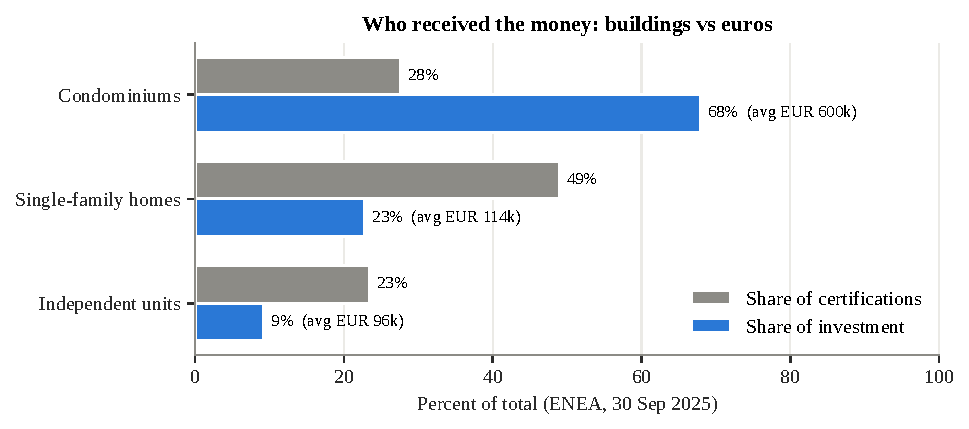
\includegraphics[width=0.86\textwidth]{../figures/fig2_composition.pdf}
\caption{Share of certifications and of investment by building type, ENEA data at 30 September 2025.}\label{fig:comp}
\end{figure}

\subsection{The footprint on the deficit}
Figure~\ref{fig:deficit} decomposes net borrowing. The orange markers show how the reclassification of the credits as payable changed the picture: the 2021 deficit, first published at 7.2\% of GDP, now stands at 8.9\%, and the 2022 figure of 8.1\% compares with a 5.6\% target \citep{agi2023}. In 2023 the building credits make up about 4 of the 7.2 points of net borrowing; the residual, 3.2\% of GDP, is close to the 3\% reference value of the EU fiscal rules. The sharp improvement in 2024, to 3.4\%, is mostly the mechanical disappearance of the credits rather than a discretionary consolidation \citep{ec2025}.

\begin{figure}[htbp]\centering
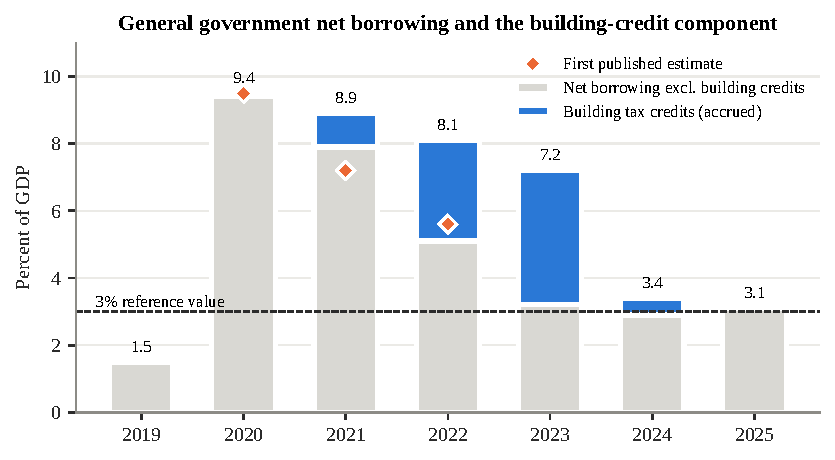
\includegraphics[width=0.86\textwidth]{../figures/fig3_deficit.pdf}
\caption{General government net borrowing, with the accrued cost of building tax credits and the first published estimates for 2020--2022. The residual is an accounting decomposition, not a counterfactual.}\label{fig:deficit}
\end{figure}

\subsection{From deficit to debt}
Figure~\ref{fig:cash} plots the output of the cash-offset model. Credits accrued at 8.5\% of GDP between 2021 and 2024 translate into cash offsets of about 2\% of GDP per year in 2024--2026, falling to around 1\% in 2027 and becoming negligible afterwards. The deficit therefore improves before the debt does. The model reproduces the qualitative pattern reported by official sources: the IMF expected tax-credit claims to be concentrated in 2024--27 \citep{imf2024}, and Istat projected the debt ratio to edge up until 2026 and to decline from 2027 as these effects fade \citep{buildnews2024}. As a rough cross-check, the model's cumulative cash cost for 2025--2027, 5.05 points of GDP, is of the same order as the 4.6 points attributed to the Parliamentary Budget Office's 2025 report in a secondary account \citep{liberi2025}.

\begin{figure}[htbp]\centering
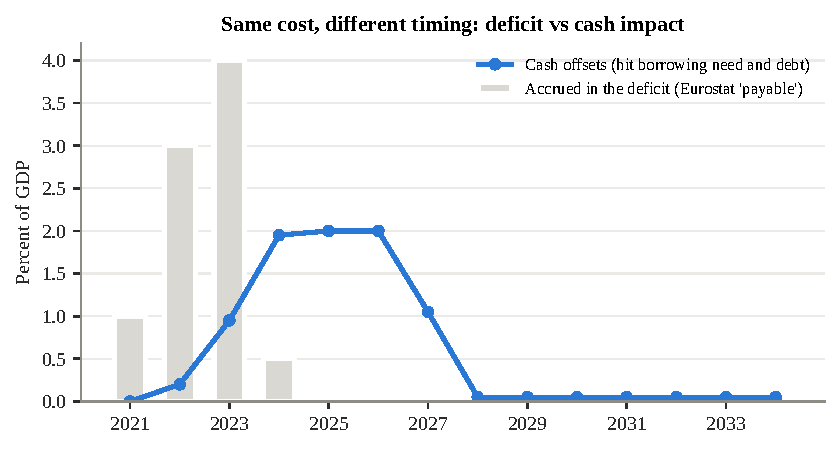
\includegraphics[width=0.86\textwidth]{../figures/fig4_cash_sim.pdf}
\caption{Accrued cost of building credits in the deficit versus the simulated cash offsets that raise the borrowing requirement. GDP held constant.}\label{fig:cash}
\end{figure}

Table~\ref{tab:sens} tests the instalment assumptions. The peak always falls in 2025, at 1.7--2.1\% of GDP, and the 2025--27 cumulative cost stays between 4.9 and 5.3 points. The main sensitivity concerns the tail: under five-year instalments, about 1 point of GDP still reaches the debt after 2027.

\begin{table}[H]\centering\small
\caption{Sensitivity of the cash profile to instalment assumptions (percent of GDP).}\label{tab:sens}
\begin{tabular}{lcccc}
\toprule
Scenario & Peak year & Peak & 2025--27 total & After 2027 \\
\midrule
Baseline (5/4/4/10 instalments) & 2025 & 2.00 & 5.05 & 0.35 \\
All vintages in 4 instalments & 2025 & 2.12 & 5.12 & 0.12 \\
All vintages in 5 instalments & 2025 & 1.70 & 4.90 & 1.00 \\
2024 vintage in 4 (no 10-year rule) & 2025 & 2.08 & 5.28 & 0.12 \\
\bottomrule
\end{tabular}
\end{table}

\subsection{The multiplier the scheme needed}
The two available counterfactual studies imply deadweight shares of 26.5\% (EUR~45 of 170 billion, Bank of Italy) and 37.6\% (EUR~70 of 186 billion, Treasury). Figure~\ref{fig:mult} maps the implied multiplier $m$ over deadweight and the effect $k$ of additional spending. With the Bank of Italy estimate, the scheme breaks even only if each additional euro of construction raised GDP by at least 1.36 euro; with the Treasury estimate the threshold rises to 1.60. The claim that the scheme would pay for itself through higher tax revenue requires $m\ge 2.34$, which in turn needs $k$ above 3.19 and 3.76 respectively.

\begin{figure}[htbp]\centering
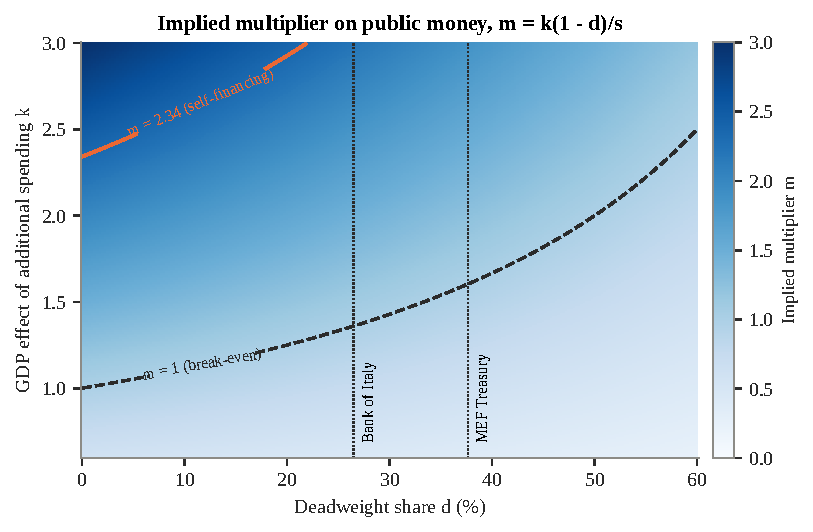
\includegraphics[width=0.84\textwidth]{../figures/fig5_multiplier.pdf}
\caption{Implied multiplier on public money as a function of the deadweight share and the GDP effect of additional spending, with $s=1$. Dashed contour: output break-even; solid contour: self-financing at a 42.7\% tax ratio. Dotted lines mark the two deadweight estimates.}\label{fig:mult}
\end{figure}

The Bank of Italy's own estimate of the multiplier is ``slightly below one'' \citep{accetturo2026}. Read through this framework, that is equivalent to saying that $k$ was below about 1.35, and it rules out self-financing by a wide margin.

\subsection{Price effects}
A subsidy that covers more than the full bill also weakens the price signal. Corsello and Ercolani estimate that the Superbonus explains about 7 of the roughly 13 points of growth in Istat's construction cost index between September 2021 and December 2023, about half of the total \citep{corsello2024,corsello2025}. Figure~\ref{fig:costs} shows the split. Part of the subsidy was therefore absorbed by higher prices paid to upstream suppliers rather than turned into additional renovation.

\begin{figure}[htbp]\centering
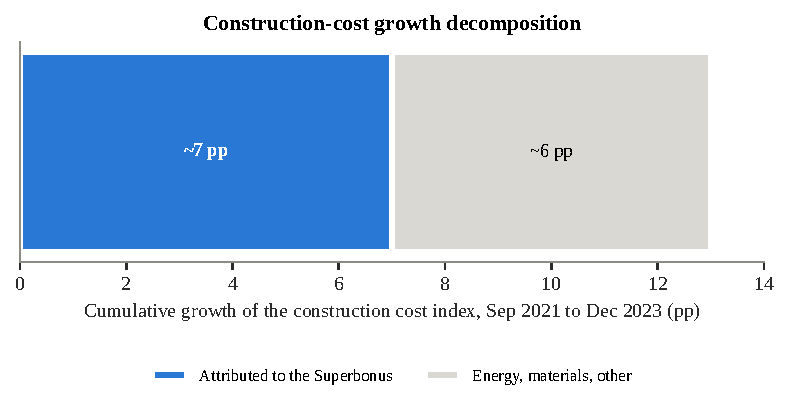
\includegraphics[width=0.84\textwidth]{../figures/fig6_costs.pdf}
\caption{Decomposition of construction-cost growth, September 2021 to December 2023, based on \citet{corsello2025}.}\label{fig:costs}
\end{figure}

\section{How the results fit the literature}
Table~\ref{tab:lit} places these results next to existing estimates, and they point the same way. The scheme did stimulate activity. The Bank of Italy finds that it accounts for the entire growth of construction value added between 2019 and 2023 \citep{accetturo2026}, and the Treasury estimates about EUR~116 billion of additional residential investment \citep{mef_wp}. Italy paid a lot for that stimulus. Estimates that report large output gains, such as the Nomisma figures of EUR~124 billion and 634,000 jobs, typically ignore deadweight and the cost of financing \citep{codogno2024}.

\begin{table}[H]\centering\small
\caption{Selected estimates of the Superbonus' economic impact.}\label{tab:lit}
\begin{tabular}{p{4.1cm}p{3.4cm}p{6.3cm}}
\toprule
Source & Type & Main finding \\
\midrule
Nomisma, via \citet{codogno2024} & Industry-sponsored & +EUR 124bn GDP, +634k jobs; no counterfactual \\
\citet{accetturo2026} & Peer-reviewed & Deadweight $>$25\% ($>$EUR 45bn); multiplier slightly below 1 \\
\citet{mef_wp} & Treasury working paper & $\approx$EUR 116bn additional investment; $\approx$EUR 70bn deadweight \\
\citet{ocpi2023} & Academic observatory & Cumulative real GDP effect $\approx$1.4\% \\
\citet{capone2026} & Peer-reviewed chapter & Most institutional multipliers below 1; only Istat's close to 1 \\
This paper & Replication-style exercise & Break-even requires $k\ge$1.36--1.60; self-financing $k\ge$3.2--3.8 \\
\bottomrule
\end{tabular}
\end{table}

Two costs are not visible in the figures. The first is fraud: transferable credits could be generated for fictitious works and sold on. By December 2025 the Guardia di Finanza reported more than EUR~9.3 billion of non-existent building and energy credits under seizure \citep{sky2025}. The second is distribution. The concentration of investment in large condominium projects (Figure~\ref{fig:comp}) is one sign of this. The Parliamentary Budget Office described a transfer from general taxpayers to higher-income owners, and only about 2\% of funds went to social housing \citep{capone2026}. Seismic subsidies were also partly capitalised into house prices, benefiting existing owners \citep{crispino2025}.

Timing mattered as well. The scheme was well suited to the 2020 recession, when construction had spare capacity, but much less so in 2022--23, when it competed with the Recovery Plan for the same firms and workers \citep{codogno2024}. A countercyclical tool extended into the upswing becomes procyclical.

\section{Limitations}
The exercises are descriptive and deliberately simple. The deficit decomposition subtracts the credits mechanically and ignores their effect on GDP and revenue. The cash-offset model holds GDP constant, assumes that holders use credits as soon as allowed and ignores the later splitting of some instalments, so its numbers describe timing rather than forecasting debt. The break-even analysis depends on a blended subsidy rate and on deadweight estimates that come from synthetic-control studies sensitive to the choice of comparison countries. Finally, the ENEA series changes definition over time, and several values are taken from press reports of official releases rather than from the original documents. Two extensions would help most: rebuilding the take-up series from ENEA's monthly reports, and estimating $k$ directly with input--output tables.

\section{Conclusion and lessons for policy}
The Superbonus raised construction activity at a very high cost. Its accrued cost explains most of Italy's deficit in 2022--23, and a simple cash model shows why the bill reaches public debt years later, at about 2\% of GDP per year in 2024--26. Given the deadweight estimated by the Bank of Italy and the Treasury, the scheme could only have broken even if each additional euro of construction had raised GDP by more than 1.36--1.60 euro, and it could only have paid for itself with a multiplier above 2.3, and no available estimate comes close to that.

In my reading, the goal was sound and the instrument was not. Future housing policy can keep the objectives of energy efficiency and seismic safety while avoiding the Superbonus' mistakes: keep a co-payment so that beneficiaries care about price, scale support to expected energy savings and to income, combine tax deductions with direct grants and access to credit, and set a budget ceiling with identified funding \citep{deblasio2024}.

\medskip
\textit{Data and code: \href{https://github.com/ettoremancuso/superbonus-fiscal-footprint}{github.com/ettoremancuso/superbonus-fiscal-footprint}.}

\renewcommand{\refname}{References}
\begin{thebibliography}{99}\small\setlength{\itemsep}{2pt}
\bibitem[Accetturo et al.(2026)]{accetturo2026} Accetturo, A., Olivieri, E. and Renzi, F. (2026). Incentives for dwelling renovations: evidence from a large fiscal programme. \textit{Fiscal Studies}, 47(1), 69--87. Earlier version: Bank of Italy, Questioni di Economia e Finanza No.~860 (2024).
\bibitem[AGI(2023)]{agi2023} AGI (2023). Effetto superbonus sui conti pubblici. \textit{Agenzia Italia}, 1 March 2023.
\bibitem[BuildNews(2024)]{buildnews2024} BuildNews (2024). Superbonus e DEF 2024, l'audizione dell'Istat. 30 April 2024.
\bibitem[Capone and Stagnaro(2026)]{capone2026} Capone, L. and Stagnaro, C. (2026). Italy's Superbonus and the capture of climate policy by Modern Monetary Theory. In Henrekson, M., Sandström, C. and Stenkula, M. (eds.), \textit{A Green Entrepreneurial State?}, 241--255. Springer, Cham.
\bibitem[Codogno(2024)]{codogno2024} Codogno, L. (2024). Italy's Superbonus 110\%: messing up with demand stimulus and the need to reinvent fiscal policy. IMK Study No.~93, Hans-Böckler-Stiftung.
\bibitem[Corsello and Ercolani(2024)]{corsello2024} Corsello, F. and Ercolani, V. (2024). The role of the Superbonus in the growth of Italian construction costs. Bank of Italy, Questioni di Economia e Finanza No.~903.
\bibitem[Corsello and Ercolani(2025)]{corsello2025} Corsello, F. and Ercolani, V. (2025). The impact of the Superbonus on Italian construction costs. \textit{VoxEU/CEPR}, 9 February 2025.
\bibitem[Council of the EU(2025)]{ec2025} Council of the European Union (2025). Country Report Italy 2025, doc. ST 9846/25 ADD 1. Brussels.
\bibitem[Crispino and Loberto(2025)]{crispino2025} Crispino, M. and Loberto, M. (2025). Bridging policy and prices: causal evidence of housing renovation subsidies on property values in Italy. \textit{Regional Science and Urban Economics}, 112, 104095.
\bibitem[de Blasio et al.(2024)]{deblasio2024} de Blasio, G. et al. (2024). Improving the energy efficiency of homes in Italy: the state of the art and some considerations for public intervention. Bank of Italy, Questioni di Economia e Finanza No.~845.
\bibitem[Edilportale(2025)]{edilportale2025} Edilportale (2025). Superbonus: superati i 127 miliardi di detrazioni maturate. 22 October 2025.
\bibitem[IMF(2024)]{imf2024} International Monetary Fund (2024). Italy: 2024 Article IV Consultation. IMF Country Report No.~24/240.
\bibitem[Istat(2023a)]{istat2023conti} Istat (2023a). Conti economici nazionali, anni 2020--2022. Press release, 22 September 2023.
\bibitem[Istat(2023b)]{istat2023eurostat} Istat (2023). Superbonus, il parere Eurostat. Press note, 26 September 2023.
\bibitem[Liberi oltre le illusioni(2025)]{liberi2025} Liberi oltre le illusioni (2025). Superbonus: cosa dice realmente il Rapporto UPB 2025? 23 June 2025.
\bibitem[MEF(n.d.)]{mef_wp} Ministry of Economy and Finance, Department of the Treasury (n.d.). The effects of tax incentives for dwelling renovations: the case of Italy. Working Paper, Rome.
\bibitem[OCPI(2023)]{ocpi2023} Osservatorio sui Conti Pubblici Italiani (2023). Gli effetti del superbonus 110\% sull'economia e sul bilancio pubblico. Università Cattolica del Sacro Cuore.
\bibitem[Sky TG24(2025)]{sky2025} Sky TG24 (2025). Frodi Superbonus, sequestrati 9,3 mld per finti crediti. 11 December 2025.
\bibitem[UPB(2024)]{upb2024} Ufficio parlamentare di bilancio (2024). Audizione sul Documento di economia e finanza 2024. 22 April 2024.
\end{thebibliography}
\end{document}
